% DAFN24 - Robotics - Lecture 2
% Roberto Masocco <roberto.masocco@uniroma2.it>
% May 10, 2024

\documentclass[aspectratio=169]{beamer}

% Slides layout
\usepackage[
    title={ROS 2},
    subtitle={Workflow and basic communication},
    event={DAFN},
    author={Roberto Masocco},
    longauthor={Roberto Masocco},
    email={roberto.masocco@uniroma2.it},
    institute={Tor Vergata},
    longinstitute={University of Rome Tor Vergata},
    department={Department of Civil Engineering and Computer Science Engineering},
    researchgroup={},
    date={May 10, 2024}
]{utvengbeamer}

% Code listings settings
\usepackage[nomath]{lmodern}
\definecolor{codegreen}{rgb}{0 0.5 0}
\definecolor{codered}{rgb}{1 0 0}
\definecolor{codeocher}{rgb}{0.8 0.47 0.13}
\usepackage{listings}
\lstdefinestyle{beamer}{
    basicstyle=\ttfamily\small,
    commentstyle=\color{codegreen},
    breakatwhitespace=false,
    captionpos=b,
    frame=lines,
    keepspaces=true,
    keywordstyle=\color{codered}\bfseries,
    numbers=left,
    numbersep=5pt,
    numberstyle=\footnotesize,
    showspaces=false,
    showstringspaces=false,
    showtabs=false,
    stringstyle=\color{codeocher},
    tabsize=2
}
\lstset{style=beamer}
\lstdefinelanguage{ros2msg}{
  alsoletter={[, ], _, /},
  morecomment=[l][\color{codegreen}]{\#},
  morekeywords={int64, uint32, string, uint8, uint8[], std_msgs/Header}
}

\usepackage{hyperref}
\usepackage{wasysym}

\begin{document}

% --- Title page ---
\frame{\titlepage}

% --- Recap ---
% Recap
% Roberto Masocco <roberto.masocco@uniroma2.it>
% May 16, 2023

% --- Recap ---
\begin{frame}{Recap}
  \textbg{ROS 2} is a \textbg{DDS}-based (for now!), open-source \textbg{middleware} for the development of robotics software and \textbg{distributed} control architectures.\\
  \bigskip
  Today, it is the \textbg{de facto} standard for the development of robotic applications, and it is supported by a \textbg{vast community} of developers and researchers.\\
  \bigskip
  The \textbg{robotics industry} is evolving rapidly towards the best practices adopted in the \textbg{software industry} in the last 30 years.\\
  \bigskip
  This lecture is \href{https://github.com/robmasocco/DAFN24_Robotics_2}{\color{blue}\underline{here}}.
\end{frame}


% --- Table of contents ---
\begin{frame}
\frametitle{Roadmap}
\tableofcontents
\end{frame}

% --- Section 1 ---
% Section 1 - ROS 2 development workflow
% Roberto Masocco <roberto.masocco@uniroma2.it>
% May 10, 2024

% ### ROS 2 development workflow ###
\section{ROS 2 development workflow}
\graphicspath{{figs/section1/}}

% --- Installing ROS 2 ---
\begin{frame}{Installing ROS 2}{HOWTO}
  On \textbg{Ubuntu} systems, the easiest way to install ROS 2 Humble is through \href{https://docs.ros.org/en/humble/Installation/Ubuntu-Install-Debians.html}{\color{blue}\underline{Debian packages}}.\\
  \bigskip
  The installation steps can be summarized as follows:
  \begin{enumerate}
    \item ensure that \textbg{locales} are properly configured;
    \item \textbg{upgrade} your system (required because of some potential \href{https://github.com/ros2/ros2/issues/1272}{\color{blue}\underline{issues with \texttt{udev}}} that might break your installation \smiley);
    \item add and configure \textbg{apt repositories};
    \item \textbg{install} packages.
  \end{enumerate}
  We have a script for this: \href{https://github.com/IntelligentSystemsLabUTV/ros2-examples/blob/humble/bin/ros2_humble_install.sh}{\color{blue}\underline{\texttt{bin/ros2\_humble\_install.sh}}}.
\end{frame}
\begin{frame}{Installing ROS 2}{Sourcing the installation}
  After the installation is complete, in order to use \textbg{CLI tools} and have libraries available to \textbg{build packages}, you need to \textbg{source the installation}:\\
  \bigskip
  \texttt{source /opt/ros/humble/setup.bash} (there are also a \texttt{.zsh} and a \texttt{.sh})\\
  \bigskip
  so that your shell, and all its child processes from then on, will know the \textbg{paths} of all the \textbg{executables}, \textbg{shared objects} (libraries), and \textbg{include directories} installed by ROS 2, plus many \textbg{environment variables}.\\
  \bigskip
  Additional commands are required to set up \textbg{command line completion} and other useful environment variables.\\
  We have a script for this too: \href{https://github.com/IntelligentSystemsLabUTV/ros2-examples/blob/humble/config/ros2_cmds.sh}{\color{blue}\underline{\texttt{config/ros2\_cmds.sh}}}.\\
  Source it, then enter \texttt{ros2humble} and you're good to go!
\end{frame}

% --- Language support ---
\begin{frame}{Language support}{Low- vs high-level programming}
  Currently, ROS 2 officially supports \textbg{two programming languages}:
  \begin{itemize}
    \item \textbg{C++} (C++17 in Humble)
    \item \textbg{Python} ($\geq$3.5, 3.10 works with Humble)
  \end{itemize}
  You can develop software packages using \textbg{only one} of them, or \textbg{both} at the same time (unofficially).
\end{frame}
\begin{frame}{Language support}{Low- vs high-level programming}
  The two languages are both fully supported since they are \textbg{complementary}:
  \begin{itemize}
    \item \textbg{C++} allows to build complex software using \textbg{modern paradigms}, but also to easily access the \textbg{hardware}, \textbg{libraries}, and \textbg{operating system} APIs when required, and to \textbg{optimize} the code for \textbg{performance}.
    \item \textbg{Python} allows to \textbg{rapidly prototype} software, especially high-level modules, and to easily \textbg{interact} with the user and \textbg{visualize data}.
  \end{itemize}
  Note how one prioritizes other features with respect to the other, and vice versa.
  \begin{block}{}
    \centering
    \textbf{This course will focus on C++, because of its better performance, major functionalities, and widespread use in the industry and robotics development community.}
  \end{block}
  The entire \href{https://github.com/ros2/ros2cli/tree/humble}{\color{blue}\underline{\texttt{ros2cli}}} suite is written in Python, and is fully \textbg{expandable}.\\
  Python examples will still be provided and discussed whenever possible.
\end{frame}
\begin{frame}{Language support}{The build system}
  The ROS 2 build system supports both \textbg{C++} and \textbg{Python} packages through a common \textbg{package manager}: \href{https://colcon.readthedocs.io/en/released/}{\color{blue}\underline{\texttt{colcon}}} (collective construction).\\
  \bigskip
  Spawned as a child project of the ROS community, its main features are:
  \begin{itemize}
    \item organization of the \textbg{build workspace} in a set of standard directories;
    \item \textbg{isolated} builds of packages, with \textbg{no pollution} of the system;
    \item automatic \textbg{dependency resolution} and \textbg{parallel} builds;
    \item support for \textbg{C}/\textbg{C++} packages through \href{https://cmake.org/}{\color{blue}\underline{CMake}};
    \item support for \textbg{Python} packages through \href{https://setuptools.pypa.io/en/latest/}{\color{blue}{\underline{\texttt{setuptools}}}}.
  \end{itemize}
  Its configuration for a package can be found in the \texttt{package.xml} \textbg{manifest file}.
\end{frame}
\begin{frame}{Language support}{CMake}
  \begin{columns}
    \column{.5\textwidth}
    CMake is a \textbg{cross-platform} build configuration generator, which allows to build software using a \textbg{single}, \textbg{unified syntax} on all supported platforms.\\
    Remember \textbg{Makefiles}? CMake is a compiler-agnostic \textbg{Makefile generator}.\\
    \bigskip
    We will write \textbg{\texttt{CMakeLists.txt}} files, which are essentially \textbg{scripts} that tell CMake how to build our software.\\
    \bigskip
    ROS 2 extends CMake with a set of \textbg{macros} and \textbg{functions}: the \href{https://docs.ros.org/en/humble/How-To-Guides/Ament-CMake-Documentation.html}{\color{blue}{\underline{\texttt{ament}}}} library.

    \column{.5\textwidth}
    \begin{figure}
      \centering
      
\includegraphics[width=.7\textwidth]{cmake}
      \caption{CMake logo.}
      \label{fig:cmake}
    \end{figure}
  \end{columns}
\end{frame}
\begin{frame}{Language support}{setuptools}
  \begin{columns}
    \column{.5\textwidth}
    \texttt{setuptools} is a \textbg{Python library} designed to ease the setup of Python projects, namely Python software packages.\\
    Remember nightmarish \texttt{import} issues? setuptools is a \textbg{dependency resolver}.\\
    \bigskip
    We will write:
    \begin{itemize}
      \item \textbg{\texttt{setup.py}} files, in which the \texttt{setup(...)} function specifies the package's metadata and dependencies;
      \item \textbg{\texttt{setup.cfg}} files, which specify the location of all \textbg{executable scripts} in the package.
    \end{itemize}

    \column{.5\textwidth}
    \begin{figure}
      \centering
      
\includegraphics[width=.7\textwidth]{setuptools}
      \caption{setuptools logo.}
      \label{fig:setuptools}
    \end{figure}
  \end{columns}
\end{frame}
\begin{frame}{Language support}{Building packages with colcon}
  The \texttt{colcon} command you will use the most is\\
  \bigskip
  \texttt{colcon build}\\
  \bigskip
  which builds all packages in the current workspace (\emph{i.e.}, directory and child directories).\\
  It has many options, but the most useful ones are:
  \begin{itemize}
    \item \texttt{-{}-event-handlers} to specify which \textbg{build events} to log (\emph{e.g.}, \texttt{console\_direct+});
    \item \texttt{-{}-packages-select} to specify which packages to build;
    \item \texttt{-{}-symlink-install} to \textbg{symlink} the executables into the \texttt{install/} directory, instead of copying them (useful for Python packages);
    \item \texttt{-{}-packages-up-to} to build a package and all its dependencies;
    \item \texttt{-{}-packages-ignore} to ignore a package and all its dependencies.
  \end{itemize}
\end{frame}
\begin{frame}{Language support}{A note}
  \begin{alertblock}{Beware!}
    \centering
    \textbr{During development, a good 85\% of all issues happens during integration and build.}
  \end{alertblock}
\end{frame}

% --- The workspace ---
\begin{frame}{The workspace}{Anatomy of a ROS 2 development directory}
  The organization of directories in a ROS 2 workspace is \textbg{standardized} because of \texttt{colcon}.\\
  We have, at least:
  \begin{itemize}
    \item \texttt{build/} (autogenerated), which contains the \textbg{build artifacts} of all packages;
    \item \texttt{install/} (autogenerated), which contains the \textbg{build products};
    \item \texttt{log/} (autogenerated), which contains the \textbg{build logs};
    \item \texttt{src/}, which contains the \textbg{source code} of all packages.
  \end{itemize}
  \begin{alertblock}{}
    \centering
    \textbr{If you use Git, remember to add \texttt{build/}, \texttt{install/}, and \texttt{log/} to your \texttt{.gitignore} file!}\\
    Similarily, \texttt{colcon} ignores them when recursively looking for packages to build.
  \end{alertblock}
\end{frame}
\begin{frame}{The workspace}{Package creation}
  In the beginning was\\
  \bigskip
  \texttt{ros2 pkg create <package\_name>}\\
  \bigskip
  which has way too many options. The main ones are:
  \begin{itemize}
    \item \texttt{-{}-destination-directory src/}
    \item \texttt{-{}-build-type <build\_type>} (\texttt{ament\_cmake} or \texttt{ament\_python})
    \item \texttt{-{}-dependencies <package\_name> ...}
  \end{itemize}
  Most of this stuff can be specified afterwards, eventually modifying the \texttt{package.xml} file.
\end{frame}


% --- Section 2 ---
% Section 2 - C++ bootstrap
% Roberto Masocco <roberto.masocco@uniroma2.it>
% May 10, 2024

% ### C++ bootstrap ###
\section{C++ bootstrap}
\graphicspath{{figs/section2/}}

% --- Code examples ---
\begin{frame}{Code examples}
	Find all course materials on \textbg{GitHub} at \href{https://github.com/IntelligentSystemsLabUTV/ros2-examples}{\color{blue}\underline{ros2-examples}} (\texttt{humble} branch).\\
	\bigskip
	The repository is organized as a \textbg{ROS 2 workspace} ready to be built, and intended to support \href{https://code.visualstudio.com/}{\color{blue}\underline{Visual Studio Code}} as \textbg{IDE}. Find all information in \href{https://github.com/IntelligentSystemsLabUTV/ros2-examples/blob/humble/README.md}{\color{blue}\underline{\texttt{README.md}}}.\\
	\bigskip
	It is also organized with \textbg{Docker containers} in mind, and supports the automated build of development containers in VS Code (more on this later).\\
	Such containers are based on our \href{https://github.com/IntelligentSystemsLabUTV/dua-template}{\color{blue}{\underline{\textbf{Distributed Unified Architecture}}}} project, which is part of Roberto Masocco's PhD thesis.\\
	Their inner workings are totally transparent, but if you're curious see \href{https://github.com/IntelligentSystemsLabUTV/ros2-examples/blob/humble/dua_template.md}{\color{blue}\underline{\texttt{dua\_template.md}}}.
	\begin{block}{}
		\centering
		Suggestion: clone it and checkout your own branch locally, to be still able to get and \texttt{merge} updates from remote.
	\end{block}
\end{frame}

% --- C++ fundamentals ---
\begin{frame}{C++ fundamentals}{Back to basics}
	C++ has been developed from C, and is a \textbg{compiled}, \textbg{strongly-typed} (mostly) language.\\
	Its main features began as extensions of C to support modern \textbg{object-oriented programming} and \textbg{generic programming} paradigms, but it has evolved into much more.\\
	\bigskip
	In order to get started with ROS 2, a minimal subset of its features is required.\\
	Dust off your C programming skills, then add:
	\begin{itemize}
		\item \href{https://www.geeksforgeeks.org/c-classes-and-objects/}{\color{blue}\underline{\textbf{Object-oriented programming}}}
		\item \href{https://www.geeksforgeeks.org/namespace-in-c/}{\color{blue}\underline{\textbf{Namespaces}}}
		\item \href{https://www.geeksforgeeks.org/templates-cpp/}{\color{blue}\underline{\textbf{Templates}}}
		\item \href{https://www.geeksforgeeks.org/smart-pointers-cpp/}{\color{blue}\underline{\textbf{Smart pointers}}}
	\end{itemize}
\end{frame}
\begin{frame}[fragile]{C++ fundamentals}{Object-oriented programming}
	\begin{columns}
		\column{.9\textwidth}
		% Listing: C++ OOP example
		\begin{lstlisting}[language=C++, caption=Example of definition of a C++ class.]
class MyClass : public ParentClass
{
public:
  MyClass();
  // ...
protected:
  // ...
private:
  // ...
};\end{lstlisting}
	\end{columns}
	Pay attention to \href{https://www.geeksforgeeks.org/inheritance-in-c/}{\color{blue}\underline{inheritance}} rules.
\end{frame}
\begin{frame}{C++ fundamentals}{Namespaces}
  C++ was designed to allow for the developmnent of large codebases, which integrated libraries and code from potentially different sources.\\
  \bigskip
  \textbg{Subdivision} of the \textbg{global namespace} is necessary to avoid naming collisions between multiple libraries, resolved with the \textbg{\texttt{::} operator}.\\
  It works like the dot in web URLs (\emph{e.g.}, \texttt{ing.uniroma2.it}).\\
  \bigskip
  Names may become very long, so usually they are hidden with \texttt{typedef}.
\end{frame}
\begin{frame}[fragile]{C++ fundamentals}{Namespaces}
	\begin{columns}
		\column{.9\textwidth}
		% Listings: C++ namespaces usage example
		\begin{lstlisting}[language=C++, caption=Example of namespaces usage.]
namespace MyLib {
  void foo() { /* Does something */ }
} // This is typically done for libraries

class MyClass
{
public:
  void foo() { /* Does something as well */ }
} my_obj; // Watch out for the ';'!

MyLib::foo(); // This is calling foo from MyLib!
my_obj.foo(); // This is calling foo from MyClass!\end{lstlisting}
	\end{columns}
\end{frame}
\begin{frame}[fragile]{C++ fundamentals}{Templates}
	Classes or functions whose \textbg{implementation depends on some data type}.\\
  When instantiated or called with a specific type, \textbg{the corresponding code is generated by the compiler}.
  \vspace{.5cm}
	\begin{columns}
		\column{.9\textwidth}
		% Listings: C++ template objects example
		\begin{lstlisting}[language=C++, caption=Example of objects of the template class \texttt{std::vector}.]
std::vector<int> int_vector;
std::vector<double> double_vector;\end{lstlisting}
	\end{columns}
  \vspace{.5cm}
  It is possible to write \textbg{specialized code} for a specific data type in the template definition.\\
	These too make names very long, so are usually \texttt{typedef}'d.
\end{frame}
\begin{frame}[fragile]{C++ fundamentals}{Shared pointers}
	A kind of \textbg{smart pointer} (there are also \texttt{unique} and \texttt{weak}) that also holds an \textbg{usage counter}, incremented by every function or object that is handling the pointer.\\
  \textbg{When the \texttt{shared\_ptr} is destroyed, if the counter is zero the pointed object is also destroyed and its memory deallocated.}
  \vspace{.1cm}
	\begin{columns}
		\column{.9\textwidth}
		% Listings: C++ shared pointer example
		\begin{lstlisting}[language=C++, caption=Example of shared pointer creation.]
{
  // A new scope starts here
  std::shared_ptr<rclcpp::Node> node =
    std::make_shared<rclcpp::Node>("my_node");
}
// Here the node and its pointer have been destroyed!\end{lstlisting}
	\end{columns}
  \vspace{.1cm}
	Obviously \texttt{std::shared\_ptr} is a template class.\\
  ROS 2 heavily relies on them, and the \texttt{SharedPtr} alias is frequently defined.
\end{frame}


% --- Section 3 ---
% Section 3 - Message topics
% Roberto Masocco <roberto.masocco@uniroma2.it>
% May 10, 2024

% ### Message topics ###
\section{Message topics}
\graphicspath{{figs/section3/}}

% --- ROS 2 messages ---
\begin{frame}{ROS 2 messages}
	A message is a \textbg{single DDS data packet} sent over a \textbg{topic}, from \textbg{publisher nodes} to \textbg{subscriber nodes}, with a specific \textbg{QoS policy}.
	\begin{figure}
		\centering
		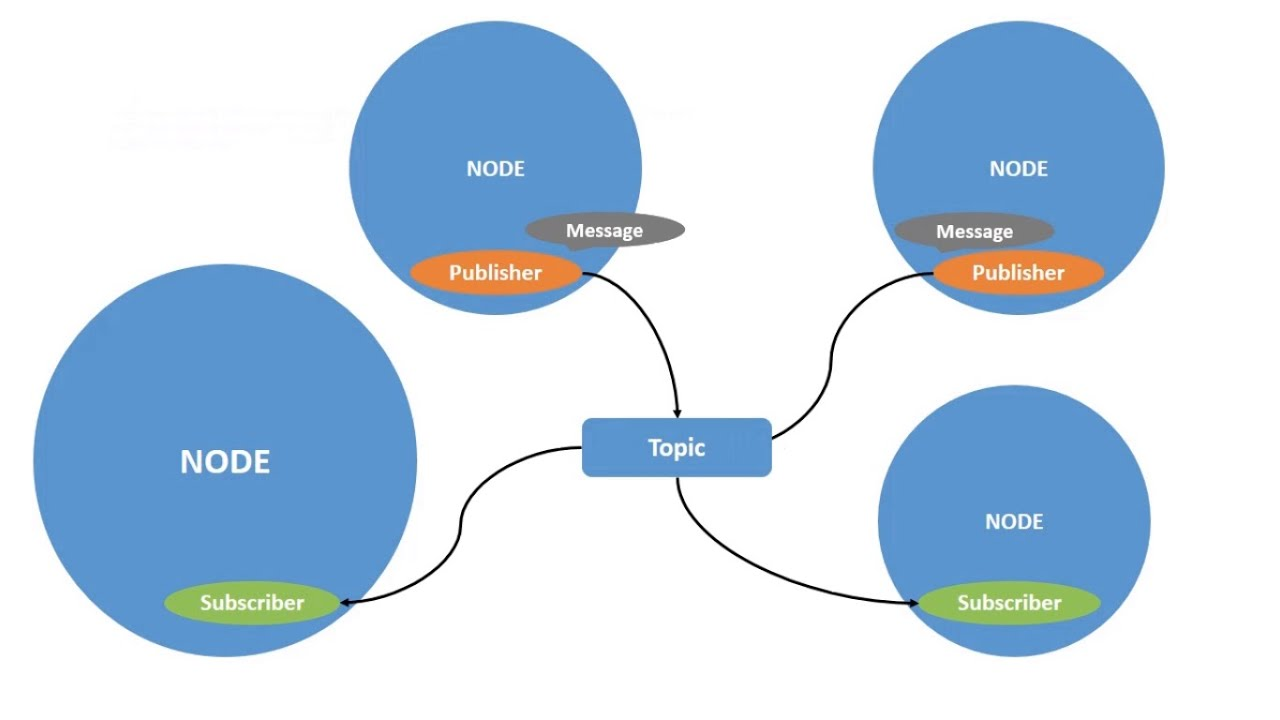
\includegraphics[scale=.16]{ros2Msg.jpg}
		\caption{Example of a topic with multiple publisher and subscriber nodes.}
		\label{fig:msg}
	\end{figure}
  Figure \ref{fig:msg} is also an example of a simple \textbg{node graph}, a pivotal concept in a distributed context.
\end{frame}

% --- Interface files - Messages ---
\begin{frame}[fragile]{Interface files}{Messages}
	Interface files format is \textbg{specified by the DDS standard}, with data types resolved to machine types according to the platform being used\footnote{\href{https://docs.ros.org/en/humble/Concepts/About-ROS-Interfaces.html}{\color{blue}\underline{About ROS 2 interfaces}} (ROS 2 Humble docs)}.\\
	Message file names end with \textbg{\texttt{.msg}}.\\
	Things start very simply...

	\begin{columns}
		\column{.9\textwidth}
		% Listing: std_msgs/msg/Int64 message definition
		\begin{lstlisting}[language=ros2msg, caption=Definition of the \texttt{std\_msgs/msg/Int64} message.]
int64 data\end{lstlisting}

		% Listing: std_msgs/msg/String message definition
		\begin{lstlisting}[language=ros2msg, caption=Definition of the \texttt{std\_msgs/msg/String} message.]
string data\end{lstlisting}
	\end{columns}

\end{frame}
\begin{frame}[fragile]{Interface files}{Messages}
	... then escalate quickly!

	\begin{columns}
		\column{.9\textwidth}
		% Listing: sensor_msgs/msg/Image
		\begin{lstlisting}[language=ros2msg, caption=Definition of the \texttt{sensor\_msgs/msg/Image} composite message.]
std_msgs/Header header

uint32 height
uint32 width

string encoding

uint8 is_bigendian
uint32 step
uint8[] data\end{lstlisting}
	\end{columns}

\end{frame}
\begin{frame}[fragile]{Interface files}{Messages}
	Special values (\emph{i.e.}, \textbg{constants}) may be specified.

	\begin{columns}
		\column{.9\textwidth}
		% Listing: message with constant
		\begin{lstlisting}[language=ros2msg, caption=Definition of an example message with a constant value.]
int64 MYNUM=1 # Must be of compatible type

int64 number\end{lstlisting}
	\end{columns}

	They are not bound to any field and will appear as \textbg{special selectable values} in the generated C++/Python libraries.\\
	ROS 2 adds its own \textbg{guidelines}\footnote{\href{https://github.com/IntelligentSystemsLabUTV/ros2-examples/blob/humble/interfaces.md}{\color{blue}\underline{ros2-examples/interfaces.md}}}, and installed interfaces can be inspected with
  \newline\newline
	\texttt{ros2 interface show}
\end{frame}

% --- Message topics - Quality of Service ---
\begin{frame}{Message topics}{Quality of Service}
	A \textbg{QoS policy} for publishers/subscribers is a data structure with the following attributes:
	\begin{itemize}
		\item \textbg{History} (\emph{keep last N} or \emph{all})
		\item \textbg{Depth} (queue size \emph{N})
		\item \textbg{Reliability} (\emph{best-effort} or \emph{reliable}, default: reliable)
		\item \textbg{Durability} (publishers resend all messages to "late-joiners")
		\item Deadline
		\item \textbg{Lifespan} (message expiration date)
		\item Liveliness
		\item Lease duration
	\end{itemize}
	Default \textbg{profiles} are available (e.g. \textbg{Sensor data}, \textbg{Service}...), see the \href{https://docs.ros.org/en/humble/Concepts/About-Quality-of-Service-Settings.html}{\color{blue}\underline{docs}}.
\end{frame}
\begin{frame}{Message topics}{Inspection tools}
  The command line tool \texttt{ros2 topic} can be used to \textbg{inspect topics} and related entities.\\
  It has a lot of \textbg{verbs}, the most important ones are:
  \begin{itemize}
    \item \texttt{list} (list all topics)
    \item \texttt{echo} (print messages to the console)
    \item \texttt{pub} (publish messages from the console)
    \item \texttt{hz} (print publishing rate and statistics)
    \item \texttt{info} (print information about a topic)
    \item \texttt{type} (print the message type)
  \end{itemize}
  each with many useful options.\\
  \textbg{Nodes} can be inspected with the \texttt{ros2 node} command, and its many verbs.
\end{frame}

% --- Example - Topic pub/sub ---
\begin{frame}{Example}{Topic pub/sub}
  \begin{block}{}
    \centering
	  Now go have a look at the \href{https://github.com/IntelligentSystemsLabUTV/ros2-examples/tree/humble/src/cpp/topic_pubsub_cpp}{\color{blue}\underline{ros2-examples/src/cpp/topic\_pubsub\_cpp}} package!
  \end{block}
\end{frame}

% --- Exercises ---
\begin{frame}{Exercises}
  \begin{itemize}
    \item Install ROS 2 on a platform of your choice.
    \item Run the \href{https://docs.ros.org/en/humble/Installation/Ubuntu-Install-Debians.html\#try-some-examples}{\color{blue}\underline{demo nodes}}.
    \item Inspect the demo topics.
    \item Interact with the demo nodes from the command line.
    \item Clone \href{https://github.com/IntelligentSystemsLabUTV/ros2-examples}{\color{blue}\underline{\texttt{ros2-examples}}} and rebuild the \texttt{topic\_pubsub\_cpp} package.
    \item Listen to the \texttt{/rosout} topic from the command line.
  \end{itemize}
\end{frame}


\end{document}
